\documentclass[11pt, a4paper]{article}

% Fonts and Encoding
\usepackage[utf8]{inputenc}
\usepackage[T1]{fontenc}
\usepackage{lmodern}

% Math and Symbols
\usepackage{amsmath, amssymb, amsthm, amsfonts, mathrsfs, mathtools}

% Layout and Geometry
\usepackage{geometry}
\geometry{a4paper, margin=1in}

% Formatting and Graphics
\usepackage{graphicx, xcolor, enumitem, booktabs, array, tabularx}

% TikZ for Illustrations
\usepackage{tikz}
\usetikzlibrary{arrows.meta, positioning, shapes.geometric, calc, backgrounds, matrix}

% Clickable Links and TOC
\usepackage{hyperref}
\hypersetup{
    colorlinks=true,
    linkcolor=blue,
    filecolor=magenta,      
    urlcolor=cyan,
    pdftitle={Advanced Mathematics Topic},
}

% Theorem Environments
\newtheorem{theorem}{Theorem}[section]
\newtheorem{lemma}[theorem]{Lemma}
\newtheorem{proposition}[theorem]{Proposition}
\newtheorem{corollary}[theorem]{Corollary}
\theoremstyle{definition}
\newtheorem{definition}{Definition}[section]
\newtheorem{axiom}{Axiom}[section]
\newtheorem{example}{Example}[section]
\theoremstyle{remark}
\newtheorem{remark}{Remark}[section]

% Custom Commands (Enforced standard notation)
\newcommand{\R}{\mathbb{R}}
\newcommand{\N}{\mathbb{N}}
\newcommand{\Z}{\mathbb{Z}}
\newcommand{\Q}{\mathbb{Q}}
\newcommand{\E}{\mathbb{E}}
\newcommand{\Prob}{\mathbb{P}}
\newcommand{\F}{\mathcal{F}}

\title{Advanced Abstract Mathematics: The Integers Modulo $n$ \\ \large Rigorous Practice Problem Set and Solutions}
\author{Tashfeen Omran}
\date{October 29, 2026}

\begin{document}

\maketitle
\tableofcontents
\newpage

\section{Concept Checklist \& Question Mapping}
\label{sec:checklist_start}
This problem set rigorously tests the abstract concepts, logical structures, and proof techniques derived from the foundational text on the Integers Modulo $n$. Every problem is mapped to a specific theoretical domain.

\begin{itemize}
    \item \textbf{C1: Algorithmic Computation \& Modular Reduction} (Problems 1, 2, 3)
    \item \textbf{C2: Set-Theoretic Properties of Equivalence Classes} (Problems 4, 5, 6)
    \item \textbf{C3: Well-Definedness of Functions on Quotient Spaces} (Problems 7, 8, 9)
    \item \textbf{C4: Zero Divisors, Integral Domains, and Prime Moduli} (Problems 10, 11, 12)
    \item \textbf{C5: Multiplicative Inverses \& Extended Euclidean Algorithm} (Problems 13, 14, 15)
    \item \textbf{C6: Solving Linear Congruences \& Systems} (Problems 16, 17, 18)
    \item \textbf{C7: Fermat's Little Theorem \& Euler's Totient Theorem} (Problems 19, 20, 21)
    \item \textbf{C8: Real-World Modeling: Linear Congruential Generators} (Problems 22, 23, 24)
    \item \textbf{C9: Real-World Modeling: Cryptography \& Hash Tables} (Problems 25, 26, 27)
    \item \textbf{C10: Advanced Diagnostic Testing (Find the Flaw)} (Problems 28, 29, 30)
\end{itemize}

\newpage

\section{Problem Statements}

\subsection{Algorithmic Computation \& Modular Reduction}
\textbf{Problem 1:} Compute the principal residue of $[7^{2026}]$ in $\Z_{11}$. \\
\textbf{Problem 2:} Find the principal residue of $[-12345]$ in $\Z_{37}$ using the Division Algorithm. \\
\textbf{Problem 3:} Evaluate the sum $[14^{28} + 15^{28}]$ in $\Z_{29}$.

\subsection{Set-Theoretic Properties of Equivalence Classes}
\textbf{Problem 4:} Let $n, m \ge 2$ be integers. Prove that if the intersection of two equivalence classes $[a]_n \cap [b]_m$ is non-empty, then $a \equiv b \pmod{\gcd(n,m)}$. \\
\textbf{Problem 5:} Let $S = \{x \in \Z : x \equiv 3 \pmod 4\}$ and $T = \{x \in \Z : x \equiv 7 \pmod 8\}$. Prove rigorously that $T \subset S$. \\
\textbf{Problem 6:} Let $p$ and $q$ be distinct prime numbers. Determine the exact number of zero divisors in the ring $\Z_{pq}$, and prove your result.

\subsection{Well-Definedness of Functions on Quotient Spaces}
\textbf{Problem 7:} Define a mapping $f: \Z_4 \to \Z_{10}$ by $f([x]_4) = [5x]_{10}$. Prove that $f$ is a well-defined function. \\
\textbf{Problem 8:} Define a mapping $g: \Z_3 \to \Z_6$ by $g([x]_3) = [x^2]_6$. Prove that $g$ is NOT well-defined. \\
\textbf{Problem 9:} Let $h: \Z_n \to \Z_m$ be defined by $h([x]_n) = [kx]_m$ for some integer $k$. Prove that $h$ is well-defined if and only if $m \mid kn$.

\subsection{Zero Divisors, Integral Domains, and Prime Moduli}
\textbf{Problem 10:} Prove that if $n > 1$ is a composite integer, then $\Z_n$ contains at least one zero divisor. \\
\textbf{Problem 11:} Prove that if $[a]$ is a zero divisor in $\Z_n$, then $[a]$ cannot have a multiplicative inverse in $\Z_n$. \\
\textbf{Problem 12:} Let $p$ be a prime number. Prove that the only elements in $\Z_p$ that are their own multiplicative inverses are $[1]$ and $[p-1]$.

\subsection{Multiplicative Inverses \& Extended Euclidean Algorithm}
\textbf{Problem 13:} Use the Extended Euclidean Algorithm to find the multiplicative inverse of $[17]$ in $\Z_{43}$. \\
\textbf{Problem 14:} Prove that the linear congruence $ax \equiv b \pmod n$ has a unique solution modulo $n$ if and only if $\gcd(a,n) = 1$. \\
\textbf{Problem 15:} Solve the system of congruences: $x \equiv 2 \pmod 5$ and $x \equiv 3 \pmod 7$.

\subsection{Solving Linear Congruences \& Systems}
\textbf{Problem 16:} Let $\gcd(a,n) = d > 1$. Prove that the congruence $ax \equiv b \pmod n$ has a solution if and only if $d \mid b$. \\
\textbf{Problem 17:} Find all distinct solutions to the congruence $12x \equiv 18 \pmod{30}$ in $\Z_{30}$. \\
\textbf{Problem 18:} Prove by exhaustion that for any integer $x$, $x^2 \not\equiv 2 \pmod 3$.

\subsection{Fermat's Little Theorem \& Euler's Totient Theorem}
\textbf{Problem 19:} Use Fermat's Little Theorem to prove that for any integer $n$, the expression $n^{13} - n$ is divisible by $2730$. \\
\textbf{Problem 20:} Use Euler's Totient Theorem to find the last two digits of $3^{400}$. \\
\textbf{Problem 21:} Prove that if $p$ and $q$ are distinct primes, then $p^{q-1} + q^{p-1} \equiv 1 \pmod{pq}$.

\subsection{Real-World Modeling: Linear Congruential Generators}
\textbf{Problem 22:} Consider a Linear Congruential Generator (LCG) defined by $X_{k+1} = (aX_k + c) \pmod m$. Let $m = 16$. Using the Hull-Dobell Theorem, find the necessary and sufficient conditions on $a$ and $c$ such that the LCG has a full period. \\
\textbf{Problem 23:} In the context of quantitative finance Monte Carlo simulations, explain rigorously why an LCG with parameters $m=2^{32}$, $a=5$, and $c=0$ fails to achieve a full period. \\
\textbf{Problem 24:} Let $U_k = \frac{X_k}{m}$ be pseudo-random variables generated by an LCG with a full period of $m$. Prove that the exact sample mean $\frac{1}{m} \sum_{k=1}^m U_k$ is equal to $\frac{m-1}{2m}$.

\subsection{Real-World Modeling: Cryptography \& Hash Tables}
\textbf{Problem 25:} In an RSA encryption scheme, the primes chosen are $p=5$ and $q=11$. Choose the smallest valid public exponent $e > 1$ and compute the corresponding private key $d$. \\
\textbf{Problem 26:} Prove that in the RSA cryptosystem, if a malicious actor discovers the value of Euler's totient function $\phi(n)$, they can efficiently factor the public modulus $n = pq$ by solving a quadratic equation. \\
\textbf{Problem 27:} A hash function for an algorithmic trading order book is defined as $h(x) = (ax + c) \pmod m$. Prove that if $\gcd(a,m) = 1$, then $h(x)$ is a bijection on $\Z_m$, guaranteeing no collisions if the domain is restricted to $m$ distinct inputs.

\subsection{Advanced Diagnostic Testing (Find the Flaw)}
\textbf{Problem 28:} Identify the logical flaw in the following proof: \textit{"Proof that $2 \equiv 0 \pmod 2$: We know $4 \equiv 2 \pmod 2$. Dividing both sides of the congruence by 2 yields $2 \equiv 1 \pmod 2$, which is false. Thus, the original premise $4 \equiv 2 \pmod 2$ must be false."} \\
\textbf{Problem 29:} Identify the mathematical flaw in the following proof: \textit{"To solve $x^2 \equiv 1 \pmod{15}$, we subtract 1 to get $x^2 - 1 \equiv 0 \pmod{15}$, which factors as $(x-1)(x+1) \equiv 0 \pmod{15}$. By the Zero Product Property, either $x-1 \equiv 0 \pmod{15}$ or $x+1 \equiv 0 \pmod{15}$. Thus, the only solutions are $x=1$ and $x=14$."} \\
\textbf{Problem 30:} Identify the theoretical flaw in the following proof: \textit{"Let $f: \Z_n \to \Z_n$ be defined by $f([x]) = [x^n]$. By Fermat's Little Theorem, $x^n \equiv x \pmod n$. Therefore, $f([x]) = [x]$ for all integers $n \ge 2$, meaning $f$ is always the identity function."}

\newpage

\section{Detailed Solutions}

\begin{proof}[Solution to Problem 1]
We wish to compute $[7^{2026}]$ in $\Z_{11}$. Since $11$ is a prime number and $\gcd(7, 11) = 1$, we apply Fermat's Little Theorem, which states that $a^{p-1} \equiv 1 \pmod p$. Thus, $7^{10} \equiv 1 \pmod{11}$. 
We divide the exponent $2026$ by $10$ using the Division Algorithm: $2026 = 10(202) + 6$.
\[ 7^{2026} = 7^{10(202) + 6} = (7^{10})^{202} \cdot 7^6 \equiv 1^{202} \cdot 7^6 \equiv 7^6 \pmod{11} \]
We reduce $7^6$ modulo $11$:
\[ 7^2 = 49 \equiv 5 \pmod{11} \]
\[ 7^6 = (7^2)^3 \equiv 5^3 = 125 \pmod{11} \]
Since $125 = 11(11) + 4$, we have $125 \equiv 4 \pmod{11}$. Therefore, $[7^{2026}] = [4]$.
\end{proof}

\begin{proof}[Solution to Problem 2]
We must find the principal residue $r$ such that $-12345 = 37q + r$, where $0 \le r < 37$. 
Dividing $-12345$ by $37$ yields approximately $-333.64$. To ensure a positive remainder, we round down the quotient to $q = -334$.
\[ -12345 = 37(-334) + r \]
\[ -12345 = -12358 + r \implies r = -12345 + 12358 = 13 \]
Thus, the principal residue is $[13]$.
\end{proof}

\begin{proof}[Solution to Problem 3]
We evaluate $[14^{28} + 15^{28}]$ in $\Z_{29}$. Since $29$ is prime, and neither $14$ nor $15$ is a multiple of $29$, we apply Fermat's Little Theorem ($a^{28} \equiv 1 \pmod{29}$).
\[ 14^{28} \equiv 1 \pmod{29} \quad \text{and} \quad 15^{28} \equiv 1 \pmod{29} \]
Summing the two congruences yields:
\[ 14^{28} + 15^{28} \equiv 1 + 1 = 2 \pmod{29} \]
Thus, the sum is $[2]$.
\end{proof}

\begin{proof}[Solution to Problem 4]
Assume $[a]_n \cap [b]_m \neq \emptyset$. Let $x \in [a]_n \cap [b]_m$. 
By definition of equivalence classes, $x \equiv a \pmod n$ and $x \equiv b \pmod m$. 
This implies there exist integers $k, j \in \Z$ such that:
\[ x = a + kn \quad \text{and} \quad x = b + jm \]
Equating the two expressions for $x$:
\[ a + kn = b + jm \implies a - b = jm - kn \]
Let $d = \gcd(n,m)$. By definition, $d \mid n$ and $d \mid m$. Therefore, $d$ divides any linear combination of $n$ and $m$, meaning $d \mid (jm - kn)$. 
Consequently, $d \mid (a - b)$, which by definition means $a \equiv b \pmod d$.
\end{proof}

\begin{proof}[Solution to Problem 5]
Let $x \in T$. By definition, $x \equiv 7 \pmod 8$, which means there exists an integer $k \in \Z$ such that $x = 7 + 8k$. 
We must show that $x \in S$, which requires showing $x \equiv 3 \pmod 4$, or $x = 3 + 4j$ for some $j \in \Z$.
We algebraically manipulate the expression for $x$:
\[ x = 7 + 8k = 3 + 4 + 8k = 3 + 4(1 + 2k) \]
Since $k \in \Z$, the term $(1 + 2k)$ is an integer. Let $j = 1 + 2k$. Then $x = 3 + 4j$, which implies $x \equiv 3 \pmod 4$. Thus, $x \in S$, proving $T \subset S$.
\end{proof}

\begin{proof}[Solution to Problem 6]
In $\Z_{pq}$, an element $[a] \neq [0]$ is a zero divisor if and only if $\gcd(a, pq) > 1$. Since $p$ and $q$ are distinct primes, the zero divisors are exactly the non-zero multiples of $p$ and the non-zero multiples of $q$.
The multiples of $p$ in $\Z_{pq}$ are $p, 2p, 3p, \dots, (q-1)p$. There are exactly $q-1$ such elements.
The multiples of $q$ in $\Z_{pq}$ are $q, 2q, 3q, \dots, (p-1)q$. There are exactly $p-1$ such elements.
Since $p$ and $q$ are distinct primes, no element (other than $0$) can be a multiple of both $p$ and $q$ within the range $1$ to $pq-1$. Thus, the sets of multiples are disjoint.
The total number of zero divisors is $(q-1) + (p-1) = p + q - 2$.
\end{proof}

\begin{proof}[Solution to Problem 7]
To prove $f([x]_4) = [5x]_{10}$ is well-defined, we must show that if $[x]_4 = [y]_4$, then $f([x]_4) = f([y]_4)$.
Assume $[x]_4 = [y]_4$. Then $x \equiv y \pmod 4$, meaning $x = y + 4k$ for some $k \in \Z$.
We evaluate $f([x]_4)$:
\[ f([x]_4) = [5x]_{10} = [5(y + 4k)]_{10} = [5y + 20k]_{10} \]
Since $20k = 10(2k)$, the term $20k$ is a multiple of $10$. Thus, $5y + 20k \equiv 5y \pmod{10}$.
\[ [5y + 20k]_{10} = [5y]_{10} = f([y]_4) \]
Since the output equivalence class is independent of the representative chosen, $f$ is well-defined.

\vspace{1em}
\begin{center}
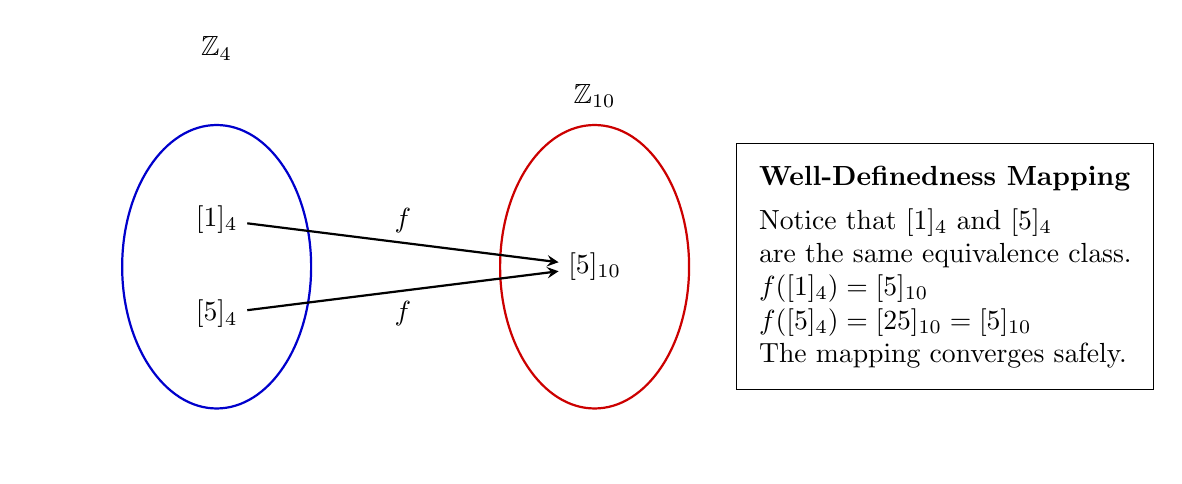
\begin{tikzpicture}[scale=1.2, >=stealth]
    % Background fill to ensure safe rendering
    \fill[white] (-2,-2) rectangle (6,2);
    
    % Sets
    \draw[thick, blue!80!black] (0,0) ellipse (1cm and 1.5cm);
    \draw[thick, red!80!black] (4,0) ellipse (1cm and 1.5cm);
    
    % Nodes in Z_4
    \node (x) at (0, 0.5) {$[1]_4$};
    \node (y) at (0, -0.5) {$[5]_4$};
    
    % Nodes in Z_10
    \node (fx) at (4, 0) {$[5]_{10}$};
    
    % Arrows
    \draw[->, thick] (x) -- (fx) node[midway, above] {$f$};
    \draw[->, thick] (y) -- (fx) node[midway, below] {$f$};
    
    % Labels
    \node[above=1.6cm of x] {$\Z_4$};
    \node[above=1.6cm of fx] {$\Z_{10}$};
    
    % Legend using single node
    \node[align=left, draw, inner sep=8pt, anchor=west] at (5.5, 0) {
        \textbf{Well-Definedness Mapping}\\[4pt]
        Notice that $[1]_4$ and $[5]_4$ \\
        are the same equivalence class.\\
        $f([1]_4) = [5]_{10}$\\
        $f([5]_4) = [25]_{10} = [5]_{10}$\\
        The mapping converges safely.
    };
\end{tikzpicture}
\end{center}
\end{proof}

\begin{proof}[Solution to Problem 8]
To prove $g([x]_3) = [x^2]_6$ is not well-defined, we must find a single counterexample where $[x]_3 = [y]_3$ but $g([x]_3) \neq g([y]_3)$.
Let $x = 1$ and $y = 4$. Clearly, $1 \equiv 4 \pmod 3$, so $[1]_3 = [4]_3$.
We evaluate the function for both representatives:
\[ g([1]_3) = [1^2]_6 = [1]_6 \]
\[ g([4]_3) = [4^2]_6 = [16]_6 \]
Since $16 = 6(2) + 4$, we have $[16]_6 = [4]_6$.
Because $[1]_6 \neq [4]_6$, the output depends on the chosen representative. Thus, $g$ is NOT well-defined.
\end{proof}

\begin{proof}[Solution to Problem 9]
($\implies$) Assume $h([x]_n) = [kx]_m$ is well-defined. Then for any $x, y$ such that $[x]_n = [y]_n$, we must have $[kx]_m = [ky]_m$. 
Let $x = n$ and $y = 0$. Clearly, $[n]_n = [0]_n$. 
By well-definedness, $h([n]_n) = h([0]_n) \implies [kn]_m = [0]_m$. 
This implies $kn \equiv 0 \pmod m$, which by definition means $m \mid kn$.

($\impliedby$) Assume $m \mid kn$. Let $[x]_n = [y]_n$. Then $x = y + cn$ for some $c \in \Z$.
Evaluate $h([x]_n)$:
\[ h([x]_n) = [kx]_m = [k(y + cn)]_m = [ky + kcn]_m \]
Since $m \mid kn$, there exists an integer $j$ such that $kn = jm$. Substituting this in:
\[ [ky + c(jm)]_m = [ky + m(cj)]_m \]
Since $cj \in \Z$, $m(cj) \equiv 0 \pmod m$. Thus, $[ky + m(cj)]_m = [ky]_m = h([y]_n)$. Therefore, $h$ is well-defined.
\end{proof}

\begin{proof}[Solution to Problem 10]
Let $n > 1$ be a composite integer. By the definition of composite numbers, there exist integers $a$ and $b$ such that $n = ab$, where $1 < a < n$ and $1 < b < n$.
Consider the equivalence classes $[a]$ and $[b]$ in $\Z_n$. Because $1 < a < n$ and $1 < b < n$, neither $a$ nor $b$ is a multiple of $n$. Thus, $[a] \neq [0]$ and $[b] \neq [0]$.
However, we evaluate their product in $\Z_n$:
\[ [a][b] = [ab] = [n] = [0] \]
Since we have found two non-zero elements whose product is zero, $[a]$ and $[b]$ are zero divisors. Thus, $\Z_n$ contains at least one zero divisor.
\end{proof}

\begin{proof}[Solution to Problem 11]
We proceed by contradiction. Suppose $[a]$ is a zero divisor in $\Z_n$ and that $[a]$ also has a multiplicative inverse, denoted $[a]^{-1}$.
Because $[a]$ is a zero divisor, there exists some non-zero element $[b] \neq [0]$ such that $[a][b] = [0]$.
We multiply both sides of this equation by the assumed inverse $[a]^{-1}$:
\[ [a]^{-1}([a][b]) = [a]^{-1}[0] \]
By associativity of multiplication in $\Z_n$:
\[ ([a]^{-1}[a])[b] = [0] \]
By the definition of an inverse, $[a]^{-1}[a] = [1]$:
\[ [1][b] = [0] \implies [b] = [0] \]
This contradicts the premise that $[b] \neq [0]$. Therefore, a zero divisor cannot have a multiplicative inverse.
\end{proof}

\begin{proof}[Solution to Problem 12]
Let $[x] \in \Z_p$ be its own multiplicative inverse. This means $[x][x] = [1]$, or $x^2 \equiv 1 \pmod p$.
This implies $p \mid (x^2 - 1)$. Factoring the expression yields $p \mid (x - 1)(x + 1)$.
By Euclid's Lemma, since $p$ is prime, if $p$ divides a product, it must divide at least one of the factors. Thus:
\[ p \mid (x - 1) \quad \text{or} \quad p \mid (x + 1) \]
If $p \mid (x - 1)$, then $x \equiv 1 \pmod p$, meaning $[x] = [1]$.
If $p \mid (x + 1)$, then $x \equiv -1 \pmod p$. In $\Z_p$, $[-1] = [p - 1]$.
Thus, the only elements that are their own inverses are $[1]$ and $[p-1]$.
\end{proof}

\begin{proof}[Solution to Problem 13]
We wish to find $x$ such that $17x \equiv 1 \pmod{43}$. We apply the Euclidean Algorithm to $43$ and $17$:
\begin{align*}
43 &= 2(17) + 9 \\
17 &= 1(9) + 8 \\
9 &= 1(8) + 1
\end{align*}
Now, we use the Extended Euclidean Algorithm by back-substituting to express $1$ as a linear combination of $17$ and $43$:
\begin{align*}
1 &= 9 - 1(8) \\
1 &= 9 - 1(17 - 1(9)) = 2(9) - 17 \\
1 &= 2(43 - 2(17)) - 17 = 2(43) - 4(17) - 17 \\
1 &= 2(43) - 5(17)
\end{align*}
Taking this equation modulo $43$ yields:
\[ -5(17) \equiv 1 \pmod{43} \]
Thus, the inverse is $[-5]$. To find the principal residue, we add $43$: $-5 + 43 = 38$. The multiplicative inverse is $[38]$.
\end{proof}

\begin{proof}[Solution to Problem 14]
($\impliedby$) Assume $\gcd(a,n) = 1$. By Bézout's Identity, there exist integers $x_0, y_0$ such that $ax_0 + ny_0 = 1$. Multiplying by $b$ gives $a(bx_0) + n(by_0) = b$. Taking this modulo $n$ yields $a(bx_0) \equiv b \pmod n$. Thus, $x = bx_0$ is a solution. To prove uniqueness, suppose $ax_1 \equiv b$ and $ax_2 \equiv b$. Then $ax_1 \equiv ax_2 \pmod n$. Since $\gcd(a,n)=1$, $a$ has an inverse. Multiplying by $a^{-1}$ yields $x_1 \equiv x_2 \pmod n$.

($\implies$) Assume $ax \equiv b \pmod n$ has a unique solution. Suppose for contradiction $\gcd(a,n) = d > 1$. If a solution $x_0$ exists, then $ax_0 - ny = b$. Consider $x_1 = x_0 + \frac{n}{d}$. 
\[ ax_1 = a\left(x_0 + \frac{n}{d}\right) = ax_0 + \frac{an}{d} \]
Since $d \mid a$, $\frac{a}{d}$ is an integer $k$. Thus $ax_1 = ax_0 + kn \equiv ax_0 \equiv b \pmod n$. Since $0 < \frac{n}{d} < n$, $x_1 \not\equiv x_0 \pmod n$, contradicting uniqueness. Thus, $d=1$.
\end{proof}

\begin{proof}[Solution to Problem 15]
We solve $x \equiv 2 \pmod 5$ and $x \equiv 3 \pmod 7$.
From the first congruence, $x = 2 + 5k$ for some $k \in \Z$.
Substitute this into the second congruence:
\[ 2 + 5k \equiv 3 \pmod 7 \implies 5k \equiv 1 \pmod 7 \]
We need the inverse of $5$ modulo $7$. Since $5(3) = 15 \equiv 1 \pmod 7$, the inverse is $3$.
Multiply by $3$:
\[ k \equiv 3 \pmod 7 \implies k = 3 + 7j \quad \text{for some } j \in \Z \]
Substitute $k$ back into the equation for $x$:
\[ x = 2 + 5(3 + 7j) = 2 + 15 + 35j = 17 + 35j \]
Thus, the solution is $x \equiv 17 \pmod{35}$.
\end{proof}

\begin{proof}[Solution to Problem 16]
The congruence $ax \equiv b \pmod n$ is equivalent to the linear Diophantine equation $ax - ny = b$ for some integer $y$.
Let $d = \gcd(a,n)$. 
($\implies$) Assume a solution $x, y$ exists. Since $d \mid a$ and $d \mid n$, $d$ must divide any linear combination of $a$ and $n$. Therefore, $d \mid (ax - ny)$, which implies $d \mid b$.
($\impliedby$) Assume $d \mid b$. Then $b = kd$ for some integer $k$. By Bézout's Identity, there exist integers $u, v$ such that $au + nv = d$. Multiplying both sides by $k$ yields $a(uk) + n(vk) = kd = b$. Taking this modulo $n$ gives $a(uk) \equiv b \pmod n$. Thus, $x = uk$ is a valid solution.
\end{proof}

\begin{proof}[Solution to Problem 17]
We solve $12x \equiv 18 \pmod{30}$. Here, $a=12, b=18, n=30$. 
First, we find $d = \gcd(12, 30) = 6$. Since $6 \mid 18$, solutions exist, and there will be exactly $d = 6$ distinct solutions modulo $30$.
We divide the entire congruence (including the modulus) by $6$:
\[ 2x \equiv 3 \pmod 5 \]
The inverse of $2$ modulo $5$ is $3$ (since $2 \times 3 = 6 \equiv 1 \pmod 5$). Multiplying by $3$:
\[ x \equiv 9 \equiv 4 \pmod 5 \]
The base solution is $x_0 = 4$. The $6$ distinct solutions modulo $30$ are generated by $x_k = x_0 + k\left(\frac{30}{6}\right) = 4 + 5k$ for $k = 0, 1, 2, 3, 4, 5$.
The solutions are: $4, 9, 14, 19, 24, 29$.
\end{proof}

\begin{proof}[Solution to Problem 18]
We test all possible equivalence classes in $\Z_3$, which are $[0], [1], [2]$.
\begin{align*}
0^2 &= 0 \not\equiv 2 \pmod 3 \\
1^2 &= 1 \not\equiv 2 \pmod 3 \\
2^2 &= 4 \equiv 1 \not\equiv 2 \pmod 3
\end{align*}
Since no integer $x$ modulo $3$ squares to $2$, the congruence $x^2 \equiv 2 \pmod 3$ has no solutions.
\end{proof}

\begin{proof}[Solution to Problem 19]
We must show that $n^{13} - n \equiv 0 \pmod{2730}$. The prime factorization of $2730$ is $2 \times 3 \times 5 \times 7 \times 13$.
By Fermat's Little Theorem, for any prime $p$, $n^p \equiv n \pmod p$.
For $p=13$: $n^{13} \equiv n \pmod{13}$.
For $p=7$: $n^7 \equiv n \pmod 7$. We multiply the exponent: $n^{13} = n \cdot (n^6)^2$. If $7 \mid n$, $n^{13} \equiv 0 \equiv n \pmod 7$. If $7 \nmid n$, $n^6 \equiv 1 \pmod 7$, so $n \cdot 1^2 \equiv n \pmod 7$. Thus $n^{13} \equiv n \pmod 7$.
For $p=5$: $n^5 \equiv n \pmod 5 \implies n^{13} = n \cdot (n^4)^3 \equiv n \cdot 1^3 \equiv n \pmod 5$.
For $p=3$: $n^3 \equiv n \pmod 3 \implies n^{13} = n \cdot (n^2)^6 \equiv n \cdot 1^6 \equiv n \pmod 3$.
For $p=2$: $n^2 \equiv n \pmod 2 \implies n^{13} \equiv n \pmod 2$.
Since $n^{13} - n$ is divisible by $2, 3, 5, 7,$ and $13$, and these primes are pairwise coprime, it is divisible by their product, $2730$.
\end{proof}

\begin{proof}[Solution to Problem 20]
Finding the last two digits of $3^{400}$ is equivalent to evaluating $3^{400} \pmod{100}$.
Since $\gcd(3, 100) = 1$, we can apply Euler's Totient Theorem: $a^{\phi(n)} \equiv 1 \pmod n$.
We calculate $\phi(100)$. The prime factorization is $100 = 2^2 \cdot 5^2$.
\[ \phi(100) = 100 \left(1 - \frac{1}{2}\right) \left(1 - \frac{1}{5}\right) = 100 \left(\frac{1}{2}\right) \left(\frac{4}{5}\right) = 40 \]
By Euler's Theorem, $3^{40} \equiv 1 \pmod{100}$.
We rewrite the exponent: $3^{400} = (3^{40})^{10} \equiv 1^{10} \equiv 1 \pmod{100}$.
Thus, the last two digits are $01$.
\end{proof}

\begin{proof}[Solution to Problem 21]
We evaluate the expression $p^{q-1} + q^{p-1}$ modulo $p$ and modulo $q$.
Modulo $p$: Since $p \equiv 0 \pmod p$, $p^{q-1} \equiv 0 \pmod p$. Because $p$ and $q$ are distinct primes, $\gcd(q,p)=1$. By Fermat's Little Theorem, $q^{p-1} \equiv 1 \pmod p$. Thus, $p^{q-1} + q^{p-1} \equiv 0 + 1 \equiv 1 \pmod p$.
Modulo $q$: Symmetrically, $q^{p-1} \equiv 0 \pmod q$, and $p^{q-1} \equiv 1 \pmod q$. Thus, $p^{q-1} + q^{p-1} \equiv 1 + 0 \equiv 1 \pmod q$.
Since the expression is congruent to $1$ modulo both $p$ and $q$, and $\gcd(p,q)=1$, it is congruent to $1$ modulo $pq$.
\end{proof}

\begin{proof}[Solution to Problem 22]
By the Hull-Dobell Theorem, an LCG $X_{k+1} = (aX_k + c) \pmod m$ has a full period if and only if:
1. $\gcd(c, m) = 1$.
2. $p \mid (a - 1)$ for all prime factors $p$ of $m$.
3. $4 \mid (a - 1)$ if $4 \mid m$.
Here, $m = 16 = 2^4$.
Condition 1: $\gcd(c, 16) = 1 \implies c$ must be an odd integer.
Condition 2: The only prime factor of $16$ is $2$. Thus, $2 \mid (a - 1) \implies a - 1$ is even $\implies a$ is odd.
Condition 3: Since $4 \mid 16$, we must have $4 \mid (a - 1) \implies a \equiv 1 \pmod 4$.
Therefore, the LCG has a full period if and only if $c$ is odd and $a \equiv 1 \pmod 4$.
\end{proof}

\begin{proof}[Solution to Problem 23]
The LCG parameters are $m = 2^{32}$, $a = 5$, and $c = 0$. 
To achieve a full period, the Hull-Dobell Theorem mandates that $\gcd(c, m) = 1$. 
Here, $\gcd(0, 2^{32}) = 2^{32} \neq 1$. 
Because $c=0$, if the seed $X_0 = 0$, the generator will perpetually output $0$, resulting in a period of $1$. Even for $X_0 \neq 0$, the sequence will eventually fall into a sub-cycle strictly smaller than $2^{32}$. Thus, it fails the full period requirement.
\end{proof}

\begin{proof}[Solution to Problem 24]
If the LCG has a full period of $m$, the sequence $\{X_1, X_2, \dots, X_m\}$ is exactly a permutation of the set $\{0, 1, 2, \dots, m-1\}$.
The sample mean of $U_k$ is:
\[ \frac{1}{m} \sum_{k=1}^m U_k = \frac{1}{m} \sum_{k=1}^m \frac{X_k}{m} = \frac{1}{m^2} \sum_{j=0}^{m-1} j \]
Using the arithmetic sum formula $\sum_{j=0}^{m-1} j = \frac{(m-1)m}{2}$:
\[ \frac{1}{m^2} \left( \frac{(m-1)m}{2} \right) = \frac{m-1}{2m} \]
\end{proof}

\begin{proof}[Solution to Problem 25]
The modulus is $n = pq = 5 \times 11 = 55$.
Euler's totient is $\phi(n) = (p-1)(q-1) = 4 \times 10 = 40$.
We must choose a public exponent $e > 1$ such that $\gcd(e, 40) = 1$. The smallest such integer is $e = 3$.
We must find the private key $d$ such that $ed \equiv 1 \pmod{40}$, meaning $3d \equiv 1 \pmod{40}$.
We can solve this by testing multiples of $40$ plus $1$: $41$ (not divisible by 3), $81$ (divisible by 3).
$3d = 81 \implies d = 27$.
Thus, the public key is $(3, 55)$ and the private key is $27$.
\end{proof}

\begin{proof}[Solution to Problem 26]
In RSA, $n = pq$ and $\phi(n) = (p-1)(q-1)$. Expanding the totient function yields:
\[ \phi(n) = pq - p - q + 1 = n - (p + q) + 1 \]
Since the attacker knows $n$ and $\phi(n)$, they can compute the sum of the primes:
\[ p + q = n - \phi(n) + 1 \]
Let $S = p + q$ and $P = pq = n$. The primes $p$ and $q$ are the roots of the quadratic equation:
\[ x^2 - Sx + P = 0 \]
By the quadratic formula, $x = \frac{S \pm \sqrt{S^2 - 4P}}{2}$. Since $S$ and $P$ are known constants, the attacker can compute $p$ and $q$ in $O(1)$ arithmetic operations, breaking the encryption.
\end{proof}

\begin{proof}[Solution to Problem 27]
To prove $h(x) = (ax + c) \pmod m$ is a bijection on $\Z_m$, we first prove it is injective (one-to-one).
Assume $h(x) = h(y)$. Then:
\[ ax + c \equiv ay + c \pmod m \implies ax \equiv ay \pmod m \]
Since $\gcd(a,m) = 1$, $a$ has a multiplicative inverse $a^{-1}$ in $\Z_m$. Multiplying both sides by $a^{-1}$ yields:
\[ x \equiv y \pmod m \]
Thus, $h$ is injective. Since the domain and codomain are the same finite set $\Z_m$, any injective function is automatically surjective (onto). Therefore, $h(x)$ is a bijection, guaranteeing no collisions.
\end{proof}

\begin{proof}[Solution to Problem 28]
\textbf{The Flaw:} The proof commits the Cancellation Fallacy. In modular arithmetic, one can only divide both sides of a congruence $ax \equiv ay \pmod n$ by $a$ if $\gcd(a,n) = 1$. Here, the proof attempts to divide by $2$ modulo $2$. Since $\gcd(2,2) = 2 \neq 1$, $2$ is a zero divisor in $\Z_2$ (specifically, $2 \equiv 0 \pmod 2$). Dividing by zero is undefined, rendering the logical deduction invalid.
\end{proof}

\begin{proof}[Solution to Problem 29]
\textbf{The Flaw:} The proof falsely assumes the Zero Product Property ($ab = 0 \implies a=0$ or $b=0$) holds in $\Z_{15}$. This property only holds in integral domains (where the modulus is prime). Because $15$ is composite, $\Z_{15}$ has zero divisors. There are other valid solutions where neither factor is zero modulo $15$. For example, if $x=4$, $(4-1)(4+1) = 3 \times 5 = 15 \equiv 0 \pmod{15}$. The full set of solutions is $x \in \{1, 4, 11, 14\}$.
\end{proof}

\begin{proof}[Solution to Problem 30]
\textbf{The Flaw:} The proof misapplies Fermat's Little Theorem. The theorem states that $x^p \equiv x \pmod p$ strictly when the modulus $p$ is a \textit{prime} number. The proof attempts to generalize this to all integers $n \ge 2$. If $n$ is composite, $x^n \equiv x \pmod n$ is generally false. For example, in $\Z_4$, let $x=2$. Then $2^4 = 16 \equiv 0 \pmod 4$, but $0 \not\equiv 2 \pmod 4$.
\end{proof}

\newpage

\section{Concept Checklist \& Question Mapping (Repeated)}
\label{sec:checklist_end}
\begin{itemize}
    \item \textbf{C1: Algorithmic Computation \& Modular Reduction} (Problems 1, 2, 3)
    \item \textbf{C2: Set-Theoretic Properties of Equivalence Classes} (Problems 4, 5, 6)
    \item \textbf{C3: Well-Definedness of Functions on Quotient Spaces} (Problems 7, 8, 9)
    \item \textbf{C4: Zero Divisors, Integral Domains, and Prime Moduli} (Problems 10, 11, 12)
    \item \textbf{C5: Multiplicative Inverses \& Extended Euclidean Algorithm} (Problems 13, 14, 15)
    \item \textbf{C6: Solving Linear Congruences \& Systems} (Problems 16, 17, 18)
    \item \textbf{C7: Fermat's Little Theorem \& Euler's Totient Theorem} (Problems 19, 20, 21)
    \item \textbf{C8: Real-World Modeling: Linear Congruential Generators} (Problems 22, 23, 24)
    \item \textbf{C9: Real-World Modeling: Cryptography \& Hash Tables} (Problems 25, 26, 27)
    \item \textbf{C10: Advanced Diagnostic Testing (Find the Flaw)} (Problems 28, 29, 30)
\end{itemize}

\end{document}